\documentclass{math}

\usepackage{tikz}

\title{University Physics 1A}
\author{Alvin Lin}
\date{September 21st, 2017}

\begin{document}

\maketitle

\section*{Dynamics}
The weight of an object is equation to the force of gravity on the object.
Therefore:
\[ W = F_{grav} = mg \]

\subsubsection*{Example}
You (mass \( m \)) are skiing on a hill inclined at \( \theta \) to the
horizontal where there is no friction. Find the normal force and your
acceleration in terms of \( m \), \( \theta \), and constants. Look at limiting
cases to see if the answer makes sense, and explain your findings.
\begin{center}
  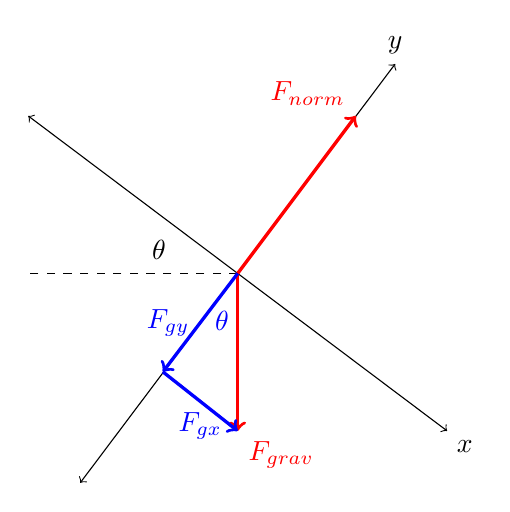
\begin{tikzpicture}
    \draw[<->] (-2,-2.66) -- (2,2.66) node[above] {\( y \)};
    \draw[<->] (-2.66,2) -- (2.66,-2) node[below right] {\( x \)};
    \draw[->,red,very thick] (0,0) -- (1.5,2) node[above left] {\( F_{norm} \)};
    \draw[->,red,very thick] (0,0) -- (0,-2) node[below right] {\( F_{grav} \)};
    \draw[dashed] node[xshift=-1cm,yshift=0.3cm] {\( \theta \)}
      (0,0) -- (-2.66,0);
    \draw[->,blue,very thick] node[xshift=-0.2cm,yshift=-0.6cm] {\( \theta \)}
      (0,0) -- (-0.95,-1.25) node[pos=0.5,left] {\( F_{gy} \)};
    \draw[->,blue,very thick] (-0.95,-1.25) -- (0,-2) node[pos=0.5,below]
      {\( F_{gx} \)};
  \end{tikzpicture}
\end{center}
\begin{center}
  \begin{tabular}{|c|c|c|}
    \hline
    & x & y \\ \hline
    \( F_{norm} \) & 0 & \( F_{norm} \) \\
    \hline
    \( F_{gravity} \) & \( mg\sin\theta \) & \( -mg\cos\theta \) \\ \hline
  \end{tabular}
\end{center}
\begin{align*}
  F_x &= 0-mg\sin\theta = ma_{x} \\
  a_x &= \frac{mg\sin\theta}{m} = g\sin\theta \\
  F_y &= F_{norm}-mg\cos\theta = 0 \\
  F_{norm} &= mg\cos\theta
\end{align*}

\subsection*{Pushing Objects}
\begin{center}
  \begin{tikzpicture}
    \draw[->] (-1,0.5) -- (-0.2,0.5) node[above left] {P};
    \draw (0,0) -- (1,0) -- (1,1) -- (0,1) -- (0,0) node[above right] {A};
    \draw (1,0) -- (3,0) -- (3,2) -- (1,2) -- (1,0) node[above right] {B};
  \end{tikzpicture}
\end{center}
Forces on Box A:
\begin{center}
  \begin{tikzpicture}
    \draw[->] (0,0) -- (1,0) node[right] {P};
    \draw[->] (0,0) -- (0,1) node[above] {\( F_{norm\ A} \)};
    \draw[->] (0,0) -- (-1,0) node[left] {\( F_{BA} \)};
    \draw[->] (0,0) -- (0,-1) node[below] {\( (m_A)g \)};
  \end{tikzpicture}
\end{center}
Forces on Box B:
\begin{center}
  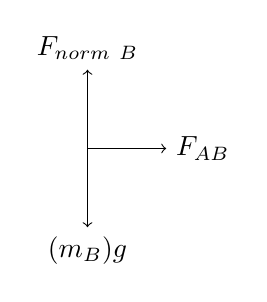
\begin{tikzpicture}
    \draw[->] (0,0) -- (1,0) node[right] {\( F_{AB} \)};
    \draw[->] (0,0) -- (0,1) node[above] {\( F_{norm\ B} \)};
    \draw[->] (0,0) -- (0,-1) node[below] {\( (m_B)g \)};
  \end{tikzpicture}
\end{center}
\begin{center}
  \begin{tabular}{|c|c|c|}
    \hline
    \textbf{Box A} & \textbf{x} & \textbf{y} \\ \hline
    gravity & 0 & \( (-m_A)g \) \\ \hline
    norm & 0 & \( F_{norm\ A} \) \\ \hline
    push & P & 0 \\ \hline
    Box B & \( -F_{BA} \) & 0 \\ \hline
    \multicolumn{3}{|c|}{} \\ \hline
    \textbf{Box B} & \textbf{x} & \textbf{y} \\ \hline
    gravity & 0 & \( (-m_B)g \) \\ \hline
    norm & 0 & \( F_{norm\ B} \) \\ \hline
    Box A & \( F_{AB} \) & 0 \\ \hline
  \end{tabular}
\end{center}
\begin{align*}
  -F_{BA}+P &= m_Aa_x \\
  F_{norm\ A}-m_Ag &= m_Aa_y = 0 \\
  F_{norm\ A} &= m_Ag \\
  F_{AB} &= m_Ba_x \\
  F_{norm\ B}-m_Bg &= m_Ba_y = 0 \\
  F_{norm\ B} &= m_Bg \\
\end{align*}
By Newton's Third Law:
\begin{align*}
  -m_Ba_x+P &= m_Aa_x \\
  P &= a_x(m_A+m_B)
\end{align*}

\section*{Reminders and Homework}
Complete the homework on TheExpertTA and WebAssign. \\
\textbf{Remember to bring the Activities Manual}

\begin{center}
  You can find all my notes at \url{http://omgimanerd.tech/notes}. If you have
  any questions, comments, or concerns, please contact me at
  alvin@omgimanerd.tech
\end{center}

\end{document}
